\documentclass[1p]{elsarticle_modified}
%\bibliographystyle{elsarticle-num}

%\usepackage[colorlinks]{hyperref}
%\usepackage{abbrmath_seonhwa} %\Abb, \Ascr, \Acal ,\Abf, \Afrak
\usepackage{amsfonts}
\usepackage{amssymb}
\usepackage{amsmath}
\usepackage{amsthm}
\usepackage{scalefnt}
\usepackage{amsbsy}
\usepackage{kotex}
\usepackage{caption}
\usepackage{subfig}
\usepackage{color}
\usepackage{graphicx}
\usepackage{xcolor} %% white, black, red, green, blue, cyan, magenta, yellow
\usepackage{float}
\usepackage{setspace}
\usepackage{hyperref}

\usepackage{tikz}
\usetikzlibrary{arrows}

\usepackage{multirow}
\usepackage{array} % fixed length table
\usepackage{hhline}

%%%%%%%%%%%%%%%%%%%%%
\makeatletter
\renewcommand*\env@matrix[1][\arraystretch]{%
	\edef\arraystretch{#1}%
	\hskip -\arraycolsep
	\let\@ifnextchar\new@ifnextchar
	\array{*\c@MaxMatrixCols c}}
\makeatother %https://tex.stackexchange.com/questions/14071/how-can-i-increase-the-line-spacing-in-a-matrix
%%%%%%%%%%%%%%%

\usepackage[normalem]{ulem}

\newcommand{\msout}[1]{\ifmmode\text{\sout{\ensuremath{#1}}}\else\sout{#1}\fi}
%SOURCE: \msout is \stkout macro in https://tex.stackexchange.com/questions/20609/strikeout-in-math-mode

\newcommand{\cancel}[1]{
	\ifmmode
	{\color{red}\msout{#1}}
	\else
	{\color{red}\sout{#1}}
	\fi
}

\newcommand{\add}[1]{
	{\color{blue}\uwave{#1}}
}

\newcommand{\replace}[2]{
	\ifmmode
	{\color{red}\msout{#1}}{\color{blue}\uwave{#2}}
	\else
	{\color{red}\sout{#1}}{\color{blue}\uwave{#2}}
	\fi
}

\newcommand{\Sol}{\mathcal{S}} %segment
\newcommand{\D}{D} %diagram
\newcommand{\A}{\mathcal{A}} %arc


%%%%%%%%%%%%%%%%%%%%%%%%%%%%%5 test

\def\sl{\operatorname{\textup{SL}}(2,\Cbb)}
\def\psl{\operatorname{\textup{PSL}}(2,\Cbb)}
\def\quan{\mkern 1mu \triangleright \mkern 1mu}

\theoremstyle{definition}
\newtheorem{thm}{Theorem}[section]
\newtheorem{prop}[thm]{Proposition}
\newtheorem{lem}[thm]{Lemma}
\newtheorem{ques}[thm]{Question}
\newtheorem{cor}[thm]{Corollary}
\newtheorem{defn}[thm]{Definition}
\newtheorem{exam}[thm]{Example}
\newtheorem{rmk}[thm]{Remark}
\newtheorem{alg}[thm]{Algorithm}

\newcommand{\I}{\sqrt{-1}}
\begin{document}

%\begin{frontmatter}
%
%\title{Boundary parabolic representations of knots up to 8 crossings}
%
%%% Group authors per affiliation:
%\author{Yunhi Cho} 
%\address{Department of Mathematics, University of Seoul, Seoul, Korea}
%\ead{yhcho@uos.ac.kr}
%
%
%\author{Seonhwa Kim} %\fnref{s_kim}}
%\address{Center for Geometry and Physics, Institute for Basic Science, Pohang, 37673, Korea}
%\ead{ryeona17@ibs.re.kr}
%
%\author{Hyuk Kim}
%\address{Department of Mathematical Sciences, Seoul National University, Seoul 08826, Korea}
%\ead{hyukkim@snu.ac.kr}
%
%\author{Seokbeom Yoon}
%\address{Department of Mathematical Sciences, Seoul National University, Seoul, 08826,  Korea}
%\ead{sbyoon15@snu.ac.kr}
%
%\begin{abstract}
%We find all boundary parabolic representation of knots up to 8 crossings.
%
%\end{abstract}
%\begin{keyword}
%    \MSC[2010] 57M25 
%\end{keyword}
%
%\end{frontmatter}

%\linenumbers
%\tableofcontents
%
\newcommand\colored[1]{\textcolor{white}{\rule[-0.35ex]{0.8em}{1.4ex}}\kern-0.8em\color{red} #1}%
%\newcommand\colored[1]{\textcolor{white}{ #1}\kern-2.17ex	\textcolor{white}{ #1}\kern-1.81ex	\textcolor{white}{ #1}\kern-2.15ex\color{red}#1	}

{\Large $\underline{11a_{114}~(K11a_{114})}$}

\setlength{\tabcolsep}{10pt}
\renewcommand{\arraystretch}{1.6}
\vspace{1cm}\begin{tabular}{m{100pt}>{\centering\arraybackslash}m{274pt}}
\multirow{5}{120pt}{
	\centering
	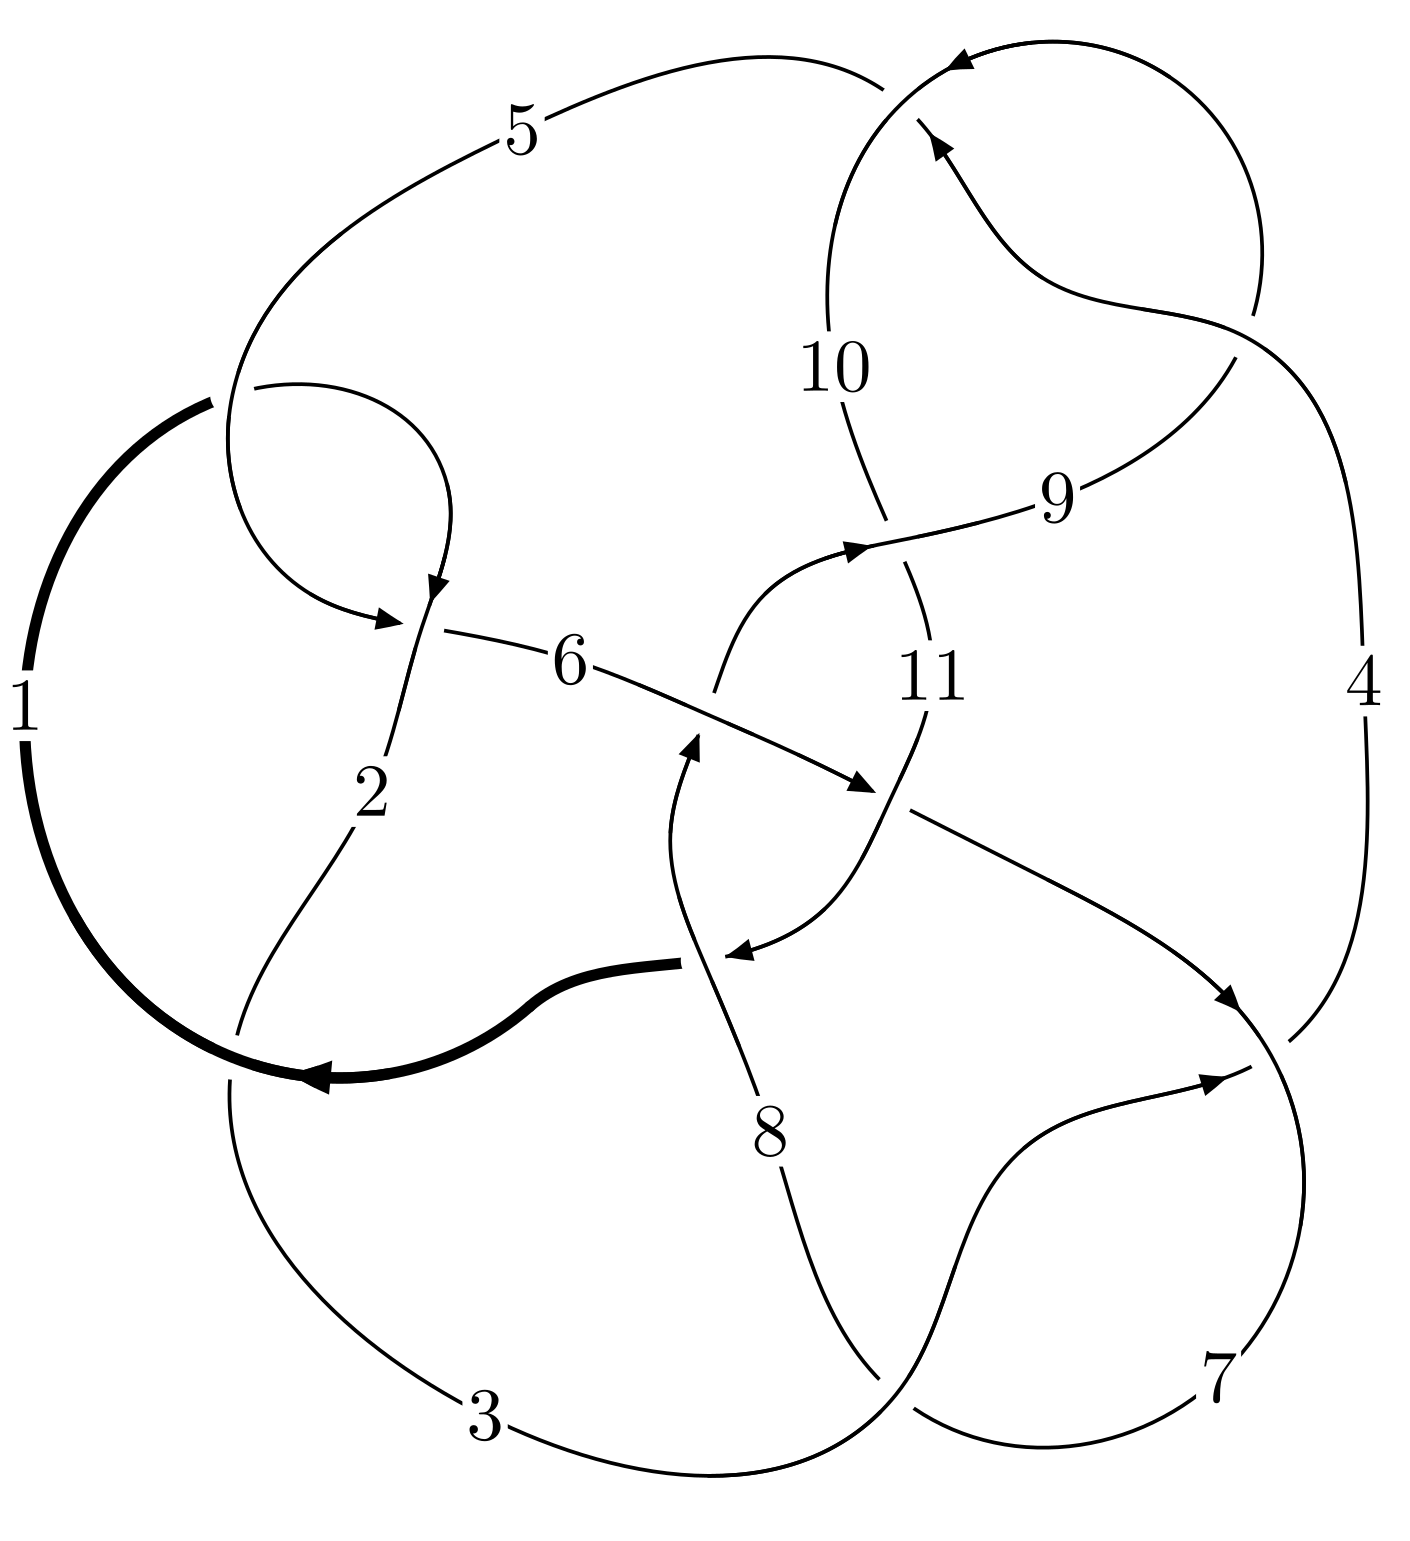
\includegraphics[width=112pt]{../../../GIT/diagram.site/Diagrams/png/363_11a_114.png}\\
\ \ \ A knot diagram\footnotemark}&
\allowdisplaybreaks
\textbf{Linearized knot diagam} \\
\cline{2-2}
 &
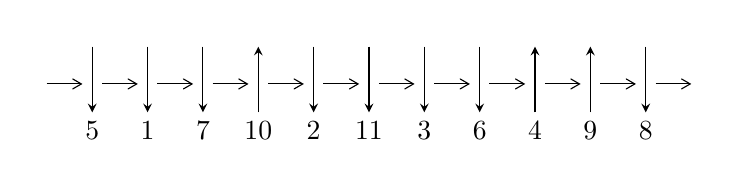
\begin{tikzpicture}[x=20pt, y=17pt]
	% nodes
	\node (C0) at (0, 0) {};
	\node (C1) at (1, 0) {};
	\node (C1U) at (1, +1) {};
	\node (C1D) at (1, -1) {5};

	\node (C2) at (2, 0) {};
	\node (C2U) at (2, +1) {};
	\node (C2D) at (2, -1) {1};

	\node (C3) at (3, 0) {};
	\node (C3U) at (3, +1) {};
	\node (C3D) at (3, -1) {7};

	\node (C4) at (4, 0) {};
	\node (C4U) at (4, +1) {};
	\node (C4D) at (4, -1) {10};

	\node (C5) at (5, 0) {};
	\node (C5U) at (5, +1) {};
	\node (C5D) at (5, -1) {2};

	\node (C6) at (6, 0) {};
	\node (C6U) at (6, +1) {};
	\node (C6D) at (6, -1) {11};

	\node (C7) at (7, 0) {};
	\node (C7U) at (7, +1) {};
	\node (C7D) at (7, -1) {3};

	\node (C8) at (8, 0) {};
	\node (C8U) at (8, +1) {};
	\node (C8D) at (8, -1) {6};

	\node (C9) at (9, 0) {};
	\node (C9U) at (9, +1) {};
	\node (C9D) at (9, -1) {4};

	\node (C10) at (10, 0) {};
	\node (C10U) at (10, +1) {};
	\node (C10D) at (10, -1) {9};

	\node (C11) at (11, 0) {};
	\node (C11U) at (11, +1) {};
	\node (C11D) at (11, -1) {8};
	\node (C12) at (12, 0) {};

	% arrows
	\draw[->,>={angle 60}]
	(C0) edge (C1) (C1) edge (C2) (C2) edge (C3) (C3) edge (C4) (C4) edge (C5) (C5) edge (C6) (C6) edge (C7) (C7) edge (C8) (C8) edge (C9) (C9) edge (C10) (C10) edge (C11) (C11) edge (C12) ;	\draw[->,>=stealth]
	(C1U) edge (C1D) (C2U) edge (C2D) (C3U) edge (C3D) (C4D) edge (C4U) (C5U) edge (C5D) (C6U) edge (C6D) (C7U) edge (C7D) (C8U) edge (C8D) (C9D) edge (C9U) (C10D) edge (C10U) (C11U) edge (C11D) ;
	\end{tikzpicture} \\
\hhline{~~} \\& 
\textbf{Solving Sequence} \\ \cline{2-2} 
 &
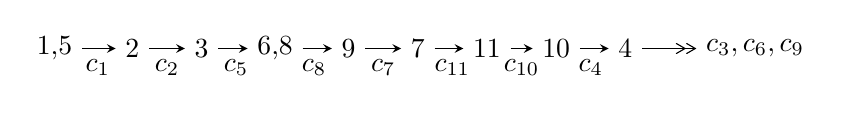
\begin{tikzpicture}[x=25pt, y=7pt]
	% node
	\node (A0) at (-1/8, 0) {1,5};
	\node (A1) at (1, 0) {2};
	\node (A2) at (2, 0) {3};
	\node (A3) at (49/16, 0) {6,8};
	\node (A4) at (33/8, 0) {9};
	\node (A5) at (41/8, 0) {7};
	\node (A6) at (49/8, 0) {11};
	\node (A7) at (57/8, 0) {10};
	\node (A8) at (65/8, 0) {4};
	\node (C1) at (1/2, -1) {$c_{1}$};
	\node (C2) at (3/2, -1) {$c_{2}$};
	\node (C3) at (5/2, -1) {$c_{5}$};
	\node (C4) at (29/8, -1) {$c_{8}$};
	\node (C5) at (37/8, -1) {$c_{7}$};
	\node (C6) at (45/8, -1) {$c_{11}$};
	\node (C7) at (53/8, -1) {$c_{10}$};
	\node (C8) at (61/8, -1) {$c_{4}$};
	\node (A9) at (10, 0) {$c_{3},c_{6},c_{9}$};

	% edge
	\draw[->,>=stealth]	
	(A0) edge (A1) (A1) edge (A2) (A2) edge (A3) (A3) edge (A4) (A4) edge (A5) (A5) edge (A6) (A6) edge (A7) (A7) edge (A8) ;
	\draw[->>,>={angle 60}]	
	(A8) edge (A9);
\end{tikzpicture} \\ 

\end{tabular} \\

\footnotetext{
The image of knot diagram is generated by the software ``\textbf{Draw programme}" developed by Andrew Bartholomew(\url{http://www.layer8.co.uk/maths/draw/index.htm\#Running-draw}), where we modified some parts for our purpose(\url{https://github.com/CATsTAILs/LinksPainter}).
}\phantom \\ \newline 
\centering \textbf{Ideals for irreducible components\footnotemark of $X_{\text{par}}$} 
 
\begin{align*}
I^u_{1}&=\langle 
-4.17956\times10^{143} u^{89}-2.07764\times10^{143} u^{88}+\cdots+4.99667\times10^{143} b-9.30374\times10^{144},\\
\phantom{I^u_{1}}&\phantom{= \langle  }3.79072\times10^{144} u^{89}+1.75627\times10^{145} u^{88}+\cdots+9.49368\times10^{144} a+8.40941\times10^{146},\\
\phantom{I^u_{1}}&\phantom{= \langle  }u^{90}-2 u^{89}+\cdots-27 u-19\rangle \\
I^u_{2}&=\langle 
u^{13}-3 u^{11}+6 u^9- u^8-7 u^7+u^6+5 u^5- u^4-2 u^3+b+2 u,\\
\phantom{I^u_{2}}&\phantom{= \langle  }5 u^{14}+3 u^{13}-15 u^{12}-7 u^{11}+35 u^{10}+11 u^9-48 u^8-11 u^7+46 u^6+5 u^5-30 u^4-4 u^3+17 u^2+a+2 u-4,\\
\phantom{I^u_{2}}&\phantom{= \langle  }u^{15}+u^{14}-3 u^{13}-3 u^{12}+7 u^{11}+6 u^{10}-10 u^9-8 u^8+10 u^7+7 u^6-7 u^5-5 u^4+4 u^3+3 u^2- u-1\rangle \\
\\
\end{align*}
\raggedright * 2 irreducible components of $\dim_{\mathbb{C}}=0$, with total 105 representations.\\
\footnotetext{All coefficients of polynomials are rational numbers. But the coefficients are sometimes approximated in decimal forms when there is not enough margin.}
\newpage
\renewcommand{\arraystretch}{1}
\centering \section*{I. $I^u_{1}= \langle -4.18\times10^{143} u^{89}-2.08\times10^{143} u^{88}+\cdots+5.00\times10^{143} b-9.30\times10^{144},\;3.79\times10^{144} u^{89}+1.76\times10^{145} u^{88}+\cdots+9.49\times10^{144} a+8.41\times10^{146},\;u^{90}-2 u^{89}+\cdots-27 u-19 \rangle$}
\flushleft \textbf{(i) Arc colorings}\\
\begin{tabular}{m{7pt} m{180pt} m{7pt} m{180pt} }
\flushright $a_{1}=$&$\begin{pmatrix}1\\0\end{pmatrix}$ \\
\flushright $a_{5}=$&$\begin{pmatrix}0\\u\end{pmatrix}$ \\
\flushright $a_{2}=$&$\begin{pmatrix}1\\u^2\end{pmatrix}$ \\
\flushright $a_{3}=$&$\begin{pmatrix}- u^2+1\\u^2\end{pmatrix}$ \\
\flushright $a_{6}=$&$\begin{pmatrix}- u\\- u^3+u\end{pmatrix}$ \\
\flushright $a_{8}=$&$\begin{pmatrix}-0.399289 u^{89}-1.84994 u^{88}+\cdots-7.29052 u-88.5790\\0.836469 u^{89}+0.415805 u^{88}+\cdots+4.57551 u+18.6199\end{pmatrix}$ \\
\flushright $a_{9}=$&$\begin{pmatrix}0.448249 u^{89}-2.43674 u^{88}+\cdots-17.3037 u-79.2582\\1.12539 u^{89}-0.745407 u^{88}+\cdots+60.6152 u+30.3562\end{pmatrix}$ \\
\flushright $a_{7}=$&$\begin{pmatrix}-0.293951 u^{89}-1.08523 u^{88}+\cdots-26.8622 u-77.8477\\0.974855 u^{89}+0.138613 u^{88}+\cdots+35.5301 u+37.1441\end{pmatrix}$ \\
\flushright $a_{11}=$&$\begin{pmatrix}1.15515 u^{89}-3.50727 u^{88}+\cdots+2.25961 u-59.7862\\0.319935 u^{89}-1.61002 u^{88}+\cdots+46.5135 u+4.38365\end{pmatrix}$ \\
\flushright $a_{10}=$&$\begin{pmatrix}1.82489 u^{89}-2.48029 u^{88}+\cdots+64.3706 u+4.28799\\-1.71061 u^{89}-1.12630 u^{88}+\cdots+89.5560 u+27.6819\end{pmatrix}$ \\
\flushright $a_{4}=$&$\begin{pmatrix}-1.07864 u^{89}+1.63188 u^{88}+\cdots+7.78149 u+61.1802\\1.34253 u^{89}-1.08046 u^{88}+\cdots-0.725013 u-7.91859\end{pmatrix}$\\ \flushright $a_{4}=$&$\begin{pmatrix}-1.07864 u^{89}+1.63188 u^{88}+\cdots+7.78149 u+61.1802\\1.34253 u^{89}-1.08046 u^{88}+\cdots-0.725013 u-7.91859\end{pmatrix}$\\&\end{tabular}
\flushleft \textbf{(ii) Obstruction class $= -1$}\\~\\
\flushleft \textbf{(iii) Cusp Shapes $= 0.323377 u^{89}-3.05080 u^{88}+\cdots+135.617 u-107.451$}\\~\\
\newpage\renewcommand{\arraystretch}{1}
\flushleft \textbf{(iv) u-Polynomials at the component}\newline \\
\begin{tabular}{m{50pt}|m{274pt}}
Crossings & \hspace{64pt}u-Polynomials at each crossing \\
\hline $$\begin{aligned}c_{1},c_{5}\end{aligned}$$&$\begin{aligned}
&u^{90}+2 u^{89}+\cdots+27 u-19
\end{aligned}$\\
\hline $$\begin{aligned}c_{2}\end{aligned}$$&$\begin{aligned}
&u^{90}+36 u^{89}+\cdots+11673 u+361
\end{aligned}$\\
\hline $$\begin{aligned}c_{3},c_{7}\end{aligned}$$&$\begin{aligned}
&u^{90}+u^{89}+\cdots+270 u-9
\end{aligned}$\\
\hline $$\begin{aligned}c_{4},c_{9}\end{aligned}$$&$\begin{aligned}
&u^{90}+u^{89}+\cdots-5 u^2+1
\end{aligned}$\\
\hline $$\begin{aligned}c_{6}\end{aligned}$$&$\begin{aligned}
&u^{90}+2 u^{89}+\cdots+33 u-1
\end{aligned}$\\
\hline $$\begin{aligned}c_{8}\end{aligned}$$&$\begin{aligned}
&u^{90}-14 u^{89}+\cdots-9 u+1
\end{aligned}$\\
\hline $$\begin{aligned}c_{10}\end{aligned}$$&$\begin{aligned}
&u^{90}-41 u^{89}+\cdots-10 u+1
\end{aligned}$\\
\hline $$\begin{aligned}c_{11}\end{aligned}$$&$\begin{aligned}
&u^{90}-8 u^{89}+\cdots+8205 u-1673
\end{aligned}$\\
\hline
\end{tabular}\\~\\
\newpage\renewcommand{\arraystretch}{1}
\flushleft \textbf{(v) Riley Polynomials at the component}\newline \\
\begin{tabular}{m{50pt}|m{274pt}}
Crossings & \hspace{64pt}Riley Polynomials at each crossing \\
\hline $$\begin{aligned}c_{1},c_{5}\end{aligned}$$&$\begin{aligned}
&y^{90}-36 y^{89}+\cdots-11673 y+361
\end{aligned}$\\
\hline $$\begin{aligned}c_{2}\end{aligned}$$&$\begin{aligned}
&y^{90}+44 y^{89}+\cdots-4387073 y+130321
\end{aligned}$\\
\hline $$\begin{aligned}c_{3},c_{7}\end{aligned}$$&$\begin{aligned}
&y^{90}+67 y^{89}+\cdots-85896 y+81
\end{aligned}$\\
\hline $$\begin{aligned}c_{4},c_{9}\end{aligned}$$&$\begin{aligned}
&y^{90}-41 y^{89}+\cdots-10 y+1
\end{aligned}$\\
\hline $$\begin{aligned}c_{6}\end{aligned}$$&$\begin{aligned}
&y^{90}+4 y^{89}+\cdots-89 y+1
\end{aligned}$\\
\hline $$\begin{aligned}c_{8}\end{aligned}$$&$\begin{aligned}
&y^{90}-4 y^{89}+\cdots+7 y+1
\end{aligned}$\\
\hline $$\begin{aligned}c_{10}\end{aligned}$$&$\begin{aligned}
&y^{90}+23 y^{89}+\cdots-198 y+1
\end{aligned}$\\
\hline $$\begin{aligned}c_{11}\end{aligned}$$&$\begin{aligned}
&y^{90}+20 y^{89}+\cdots+12841443 y+2798929
\end{aligned}$\\
\hline
\end{tabular}\\~\\
\newpage\flushleft \textbf{(vi) Complex Volumes and Cusp Shapes}
$$\begin{array}{c|c|c}  
\text{Solutions to }I^u_{1}& \I (\text{vol} + \sqrt{-1}CS) & \text{Cusp shape}\\
 \hline 
\begin{aligned}
u &= -0.872945 + 0.501934 I \\
a &= -0.353599 + 1.137060 I \\
b &= \phantom{-}1.94991 + 0.34028 I\end{aligned}
 & -1.65776 + 2.02775 I & \phantom{-0.000000 } 0 \\ \hline\begin{aligned}
u &= -0.872945 - 0.501934 I \\
a &= -0.353599 - 1.137060 I \\
b &= \phantom{-}1.94991 - 0.34028 I\end{aligned}
 & -1.65776 - 2.02775 I & \phantom{-0.000000 } 0 \\ \hline\begin{aligned}
u &= \phantom{-}0.887662 + 0.444502 I \\
a &= \phantom{-}0.35902 - 2.01369 I \\
b &= \phantom{-}0.894026 + 1.049230 I\end{aligned}
 & -1.87083 - 2.34624 I & \phantom{-0.000000 } 0 \\ \hline\begin{aligned}
u &= \phantom{-}0.887662 - 0.444502 I \\
a &= \phantom{-}0.35902 + 2.01369 I \\
b &= \phantom{-}0.894026 - 1.049230 I\end{aligned}
 & -1.87083 + 2.34624 I & \phantom{-0.000000 } 0 \\ \hline\begin{aligned}
u &= -0.736112 + 0.693083 I \\
a &= \phantom{-}0.602880 + 1.051170 I \\
b &= -0.351565 - 0.763113 I\end{aligned}
 & \phantom{-}3.42582 + 0.72145 I & \phantom{-0.000000 } 0 \\ \hline\begin{aligned}
u &= -0.736112 - 0.693083 I \\
a &= \phantom{-}0.602880 - 1.051170 I \\
b &= -0.351565 + 0.763113 I\end{aligned}
 & \phantom{-}3.42582 - 0.72145 I & \phantom{-0.000000 } 0 \\ \hline\begin{aligned}
u &= \phantom{-}0.610400 + 0.816519 I \\
a &= \phantom{-}1.10218 - 1.06449 I \\
b &= -0.82176 + 1.50141 I\end{aligned}
 & \phantom{-}8.88297 + 2.76328 I & \phantom{-0.000000 } 0 \\ \hline\begin{aligned}
u &= \phantom{-}0.610400 - 0.816519 I \\
a &= \phantom{-}1.10218 + 1.06449 I \\
b &= -0.82176 - 1.50141 I\end{aligned}
 & \phantom{-}8.88297 - 2.76328 I & \phantom{-0.000000 } 0 \\ \hline\begin{aligned}
u &= \phantom{-}0.851253 + 0.574688 I \\
a &= \phantom{-}0.238775 + 1.278400 I \\
b &= \phantom{-}0.388781 - 1.039950 I\end{aligned}
 & \phantom{-}5.10240 - 3.43208 I & \phantom{-0.000000 } 0 \\ \hline\begin{aligned}
u &= \phantom{-}0.851253 - 0.574688 I \\
a &= \phantom{-}0.238775 - 1.278400 I \\
b &= \phantom{-}0.388781 + 1.039950 I\end{aligned}
 & \phantom{-}5.10240 + 3.43208 I & \phantom{-0.000000 } 0\\
 \hline 
 \end{array}$$\newpage$$\begin{array}{c|c|c}  
\text{Solutions to }I^u_{1}& \I (\text{vol} + \sqrt{-1}CS) & \text{Cusp shape}\\
 \hline 
\begin{aligned}
u &= -0.701758 + 0.763935 I \\
a &= \phantom{-}0.087700 + 0.920133 I \\
b &= -0.305002 - 0.900231 I\end{aligned}
 & \phantom{-}3.66503 + 0.99650 I & \phantom{-0.000000 } 0 \\ \hline\begin{aligned}
u &= -0.701758 - 0.763935 I \\
a &= \phantom{-}0.087700 - 0.920133 I \\
b &= -0.305002 + 0.900231 I\end{aligned}
 & \phantom{-}3.66503 - 0.99650 I & \phantom{-0.000000 } 0 \\ \hline\begin{aligned}
u &= \phantom{-}0.857462 + 0.584959 I \\
a &= \phantom{-}1.76238 - 0.77479 I \\
b &= \phantom{-}0.495062 + 0.649066 I\end{aligned}
 & \phantom{-}5.07632 - 1.17400 I & \phantom{-0.000000 } 0 \\ \hline\begin{aligned}
u &= \phantom{-}0.857462 - 0.584959 I \\
a &= \phantom{-}1.76238 + 0.77479 I \\
b &= \phantom{-}0.495062 - 0.649066 I\end{aligned}
 & \phantom{-}5.07632 + 1.17400 I & \phantom{-0.000000 } 0 \\ \hline\begin{aligned}
u &= \phantom{-}0.774750 + 0.567973 I \\
a &= -0.19680 + 1.83254 I \\
b &= -1.87636 - 0.42388 I\end{aligned}
 & \phantom{-}2.30569 + 3.30607 I & \phantom{-0.000000 } 0 \\ \hline\begin{aligned}
u &= \phantom{-}0.774750 - 0.567973 I \\
a &= -0.19680 - 1.83254 I \\
b &= -1.87636 + 0.42388 I\end{aligned}
 & \phantom{-}2.30569 - 3.30607 I & \phantom{-0.000000 } 0 \\ \hline\begin{aligned}
u &= -0.496582 + 0.913249 I \\
a &= -0.88468 - 1.12826 I \\
b &= \phantom{-}0.73357 + 1.33284 I\end{aligned}
 & \phantom{-}3.23883 - 5.87656 I & \phantom{-0.000000 } 0 \\ \hline\begin{aligned}
u &= -0.496582 - 0.913249 I \\
a &= -0.88468 + 1.12826 I \\
b &= \phantom{-}0.73357 - 1.33284 I\end{aligned}
 & \phantom{-}3.23883 + 5.87656 I & \phantom{-0.000000 } 0 \\ \hline\begin{aligned}
u &= \phantom{-}1.006990 + 0.383697 I \\
a &= -0.990900 + 0.589869 I \\
b &= -0.128969 - 0.889913 I\end{aligned}
 & -1.94313 - 0.77906 I & \phantom{-0.000000 } 0 \\ \hline\begin{aligned}
u &= \phantom{-}1.006990 - 0.383697 I \\
a &= -0.990900 - 0.589869 I \\
b &= -0.128969 + 0.889913 I\end{aligned}
 & -1.94313 + 0.77906 I & \phantom{-0.000000 } 0\\
 \hline 
 \end{array}$$\newpage$$\begin{array}{c|c|c}  
\text{Solutions to }I^u_{1}& \I (\text{vol} + \sqrt{-1}CS) & \text{Cusp shape}\\
 \hline 
\begin{aligned}
u &= -0.621493 + 0.885684 I \\
a &= \phantom{-}0.069658 + 0.683614 I \\
b &= -0.226329 - 0.871694 I\end{aligned}
 & \phantom{-}3.75525 + 1.11582 I & \phantom{-0.000000 } 0 \\ \hline\begin{aligned}
u &= -0.621493 - 0.885684 I \\
a &= \phantom{-}0.069658 - 0.683614 I \\
b &= -0.226329 + 0.871694 I\end{aligned}
 & \phantom{-}3.75525 - 1.11582 I & \phantom{-0.000000 } 0 \\ \hline\begin{aligned}
u &= \phantom{-}0.805011 + 0.723930 I \\
a &= \phantom{-}0.000178 + 1.241640 I \\
b &= \phantom{-}0.402112 - 0.956324 I\end{aligned}
 & \phantom{-}5.11520 + 2.40414 I & \phantom{-0.000000 } 0 \\ \hline\begin{aligned}
u &= \phantom{-}0.805011 - 0.723930 I \\
a &= \phantom{-}0.000178 - 1.241640 I \\
b &= \phantom{-}0.402112 + 0.956324 I\end{aligned}
 & \phantom{-}5.11520 - 2.40414 I & \phantom{-0.000000 } 0 \\ \hline\begin{aligned}
u &= -0.913503 + 0.079203 I \\
a &= -0.501241 + 1.245300 I \\
b &= -0.705898 + 0.492074 I\end{aligned}
 & \phantom{-}2.89768 + 2.60574 I & \phantom{-0.000000 } 0 \\ \hline\begin{aligned}
u &= -0.913503 - 0.079203 I \\
a &= -0.501241 - 1.245300 I \\
b &= -0.705898 - 0.492074 I\end{aligned}
 & \phantom{-}2.89768 - 2.60574 I & \phantom{-0.000000 } 0 \\ \hline\begin{aligned}
u &= \phantom{-}0.915800\phantom{ +0.000000I} \\
a &= -0.955871\phantom{ +0.000000I} \\
b &= -0.493066\phantom{ +0.000000I}\end{aligned}
 & -1.55660\phantom{ +0.000000I} & -5.00000\phantom{ +0.000000I} \\ \hline\begin{aligned}
u &= \phantom{-}0.918511 + 0.576128 I \\
a &= \phantom{-}1.006050 + 0.579665 I \\
b &= -1.93814 + 0.98297 I\end{aligned}
 & \phantom{-}1.83988 - 7.87904 I & \phantom{-0.000000 } 0 \\ \hline\begin{aligned}
u &= \phantom{-}0.918511 - 0.576128 I \\
a &= \phantom{-}1.006050 - 0.579665 I \\
b &= -1.93814 - 0.98297 I\end{aligned}
 & \phantom{-}1.83988 + 7.87904 I & \phantom{-0.000000 } 0 \\ \hline\begin{aligned}
u &= -1.066380 + 0.198905 I \\
a &= \phantom{-}0.370881 + 0.038702 I \\
b &= \phantom{-}1.102150 + 0.474228 I\end{aligned}
 & -4.90537 + 0.82863 I & \phantom{-0.000000 } 0\\
 \hline 
 \end{array}$$\newpage$$\begin{array}{c|c|c}  
\text{Solutions to }I^u_{1}& \I (\text{vol} + \sqrt{-1}CS) & \text{Cusp shape}\\
 \hline 
\begin{aligned}
u &= -1.066380 - 0.198905 I \\
a &= \phantom{-}0.370881 - 0.038702 I \\
b &= \phantom{-}1.102150 - 0.474228 I\end{aligned}
 & -4.90537 - 0.82863 I & \phantom{-0.000000 } 0 \\ \hline\begin{aligned}
u &= \phantom{-}0.533194 + 0.973241 I \\
a &= \phantom{-}0.853278 - 1.053140 I \\
b &= -0.79058 + 1.29478 I\end{aligned}
 & \phantom{-}5.57367 + 11.40460 I & \phantom{-0.000000 } 0 \\ \hline\begin{aligned}
u &= \phantom{-}0.533194 - 0.973241 I \\
a &= \phantom{-}0.853278 + 1.053140 I \\
b &= -0.79058 - 1.29478 I\end{aligned}
 & \phantom{-}5.57367 - 11.40460 I & \phantom{-0.000000 } 0 \\ \hline\begin{aligned}
u &= -0.829414 + 0.315657 I \\
a &= -0.76244 - 2.14466 I \\
b &= -0.76353 + 1.45828 I\end{aligned}
 & \phantom{-}0.23371 - 3.50455 I & \phantom{-0.000000 } 0 \\ \hline\begin{aligned}
u &= -0.829414 - 0.315657 I \\
a &= -0.76244 + 2.14466 I \\
b &= -0.76353 - 1.45828 I\end{aligned}
 & \phantom{-}0.23371 + 3.50455 I & \phantom{-0.000000 } 0 \\ \hline\begin{aligned}
u &= \phantom{-}0.259644 + 1.086570 I \\
a &= -0.003044 + 0.482911 I \\
b &= \phantom{-}0.081154 - 0.850794 I\end{aligned}
 & \phantom{-}6.46351 + 1.09920 I & \phantom{-0.000000 } 0 \\ \hline\begin{aligned}
u &= \phantom{-}0.259644 - 1.086570 I \\
a &= -0.003044 - 0.482911 I \\
b &= \phantom{-}0.081154 + 0.850794 I\end{aligned}
 & \phantom{-}6.46351 - 1.09920 I & \phantom{-0.000000 } 0 \\ \hline\begin{aligned}
u &= \phantom{-}1.075840 + 0.314619 I \\
a &= -0.932582 - 0.563589 I \\
b &= \phantom{-}0.862432 - 0.970765 I\end{aligned}
 & -2.59949 - 0.41889 I & \phantom{-0.000000 } 0 \\ \hline\begin{aligned}
u &= \phantom{-}1.075840 - 0.314619 I \\
a &= -0.932582 + 0.563589 I \\
b &= \phantom{-}0.862432 + 0.970765 I\end{aligned}
 & -2.59949 + 0.41889 I & \phantom{-0.000000 } 0 \\ \hline\begin{aligned}
u &= -0.750139 + 0.431514 I \\
a &= -0.458402 + 1.189240 I \\
b &= -0.336805 - 1.096300 I\end{aligned}
 & \phantom{-}4.12746 - 0.06763 I & -5.00000 + 0. I\phantom{ +0.000000I}\\
 \hline 
 \end{array}$$\newpage$$\begin{array}{c|c|c}  
\text{Solutions to }I^u_{1}& \I (\text{vol} + \sqrt{-1}CS) & \text{Cusp shape}\\
 \hline 
\begin{aligned}
u &= -0.750139 - 0.431514 I \\
a &= -0.458402 - 1.189240 I \\
b &= -0.336805 + 1.096300 I\end{aligned}
 & \phantom{-}4.12746 + 0.06763 I & -5.00000 + 0. I\phantom{ +0.000000I} \\ \hline\begin{aligned}
u &= \phantom{-}1.130920 + 0.112054 I \\
a &= -0.435009 - 0.151586 I \\
b &= -0.968053 + 0.539467 I\end{aligned}
 & -4.06860 + 3.93905 I & \phantom{-0.000000 } 0 \\ \hline\begin{aligned}
u &= \phantom{-}1.130920 - 0.112054 I \\
a &= -0.435009 + 0.151586 I \\
b &= -0.968053 - 0.539467 I\end{aligned}
 & -4.06860 - 3.93905 I & \phantom{-0.000000 } 0 \\ \hline\begin{aligned}
u &= \phantom{-}0.906289 + 0.696953 I \\
a &= \phantom{-}1.34768 - 1.32182 I \\
b &= \phantom{-}0.497588 + 0.734318 I\end{aligned}
 & \phantom{-}4.80179 - 7.83323 I & \phantom{-0.000000 } 0 \\ \hline\begin{aligned}
u &= \phantom{-}0.906289 - 0.696953 I \\
a &= \phantom{-}1.34768 + 1.32182 I \\
b &= \phantom{-}0.497588 - 0.734318 I\end{aligned}
 & \phantom{-}4.80179 + 7.83323 I & \phantom{-0.000000 } 0 \\ \hline\begin{aligned}
u &= -0.893897 + 0.720474 I \\
a &= -0.347044 - 1.362470 I \\
b &= -0.675805 + 0.773415 I\end{aligned}
 & \phantom{-}2.92181 + 4.66361 I & \phantom{-0.000000 } 0 \\ \hline\begin{aligned}
u &= -0.893897 - 0.720474 I \\
a &= -0.347044 + 1.362470 I \\
b &= -0.675805 - 0.773415 I\end{aligned}
 & \phantom{-}2.92181 - 4.66361 I & \phantom{-0.000000 } 0 \\ \hline\begin{aligned}
u &= -0.481220 + 0.674909 I \\
a &= \phantom{-}0.86086 + 1.65314 I \\
b &= -0.518390 - 0.630908 I\end{aligned}
 & \phantom{-}0.76902 - 5.82157 I & -2.53875 + 6.05910 I \\ \hline\begin{aligned}
u &= -0.481220 - 0.674909 I \\
a &= \phantom{-}0.86086 - 1.65314 I \\
b &= -0.518390 + 0.630908 I\end{aligned}
 & \phantom{-}0.76902 + 5.82157 I & -2.53875 - 6.05910 I \\ \hline\begin{aligned}
u &= \phantom{-}1.022490 + 0.579602 I \\
a &= \phantom{-}0.53864 - 1.78720 I \\
b &= \phantom{-}0.648451 + 0.951250 I\end{aligned}
 & -2.49493 - 5.56780 I & \phantom{-0.000000 } 0\\
 \hline 
 \end{array}$$\newpage$$\begin{array}{c|c|c}  
\text{Solutions to }I^u_{1}& \I (\text{vol} + \sqrt{-1}CS) & \text{Cusp shape}\\
 \hline 
\begin{aligned}
u &= \phantom{-}1.022490 - 0.579602 I \\
a &= \phantom{-}0.53864 + 1.78720 I \\
b &= \phantom{-}0.648451 - 0.951250 I\end{aligned}
 & -2.49493 + 5.56780 I & \phantom{-0.000000 } 0 \\ \hline\begin{aligned}
u &= -1.063110 + 0.501451 I \\
a &= \phantom{-}1.41649 + 0.97024 I \\
b &= \phantom{-}0.32696 - 1.69396 I\end{aligned}
 & -1.39911 + 6.64640 I & \phantom{-0.000000 } 0 \\ \hline\begin{aligned}
u &= -1.063110 - 0.501451 I \\
a &= \phantom{-}1.41649 - 0.97024 I \\
b &= \phantom{-}0.32696 + 1.69396 I\end{aligned}
 & -1.39911 - 6.64640 I & \phantom{-0.000000 } 0 \\ \hline\begin{aligned}
u &= -0.988063 + 0.637660 I \\
a &= -1.028120 - 0.832488 I \\
b &= -0.568669 + 0.693404 I\end{aligned}
 & \phantom{-}2.64990 + 4.39254 I & \phantom{-0.000000 } 0 \\ \hline\begin{aligned}
u &= -0.988063 - 0.637660 I \\
a &= -1.028120 + 0.832488 I \\
b &= -0.568669 - 0.693404 I\end{aligned}
 & \phantom{-}2.64990 - 4.39254 I & \phantom{-0.000000 } 0 \\ \hline\begin{aligned}
u &= -0.965090 + 0.711279 I \\
a &= -0.65456 - 1.29507 I \\
b &= -0.612386 + 0.775291 I\end{aligned}
 & \phantom{-}2.85757 + 4.68949 I & \phantom{-0.000000 } 0 \\ \hline\begin{aligned}
u &= -0.965090 - 0.711279 I \\
a &= -0.65456 + 1.29507 I \\
b &= -0.612386 - 0.775291 I\end{aligned}
 & \phantom{-}2.85757 - 4.68949 I & \phantom{-0.000000 } 0 \\ \hline\begin{aligned}
u &= -1.051130 + 0.615181 I \\
a &= -0.59658 - 1.78715 I \\
b &= -0.610037 + 0.942966 I\end{aligned}
 & -0.84298 + 10.85530 I & \phantom{-0.000000 } 0 \\ \hline\begin{aligned}
u &= -1.051130 - 0.615181 I \\
a &= -0.59658 + 1.78715 I \\
b &= -0.610037 - 0.942966 I\end{aligned}
 & -0.84298 - 10.85530 I & \phantom{-0.000000 } 0 \\ \hline\begin{aligned}
u &= -1.108590 + 0.519036 I \\
a &= \phantom{-}0.828820 + 0.255791 I \\
b &= -0.373453 - 0.967630 I\end{aligned}
 & -0.97957 + 6.41665 I & \phantom{-0.000000 } 0\\
 \hline 
 \end{array}$$\newpage$$\begin{array}{c|c|c}  
\text{Solutions to }I^u_{1}& \I (\text{vol} + \sqrt{-1}CS) & \text{Cusp shape}\\
 \hline 
\begin{aligned}
u &= -1.108590 - 0.519036 I \\
a &= \phantom{-}0.828820 - 0.255791 I \\
b &= -0.373453 + 0.967630 I\end{aligned}
 & -0.97957 - 6.41665 I & \phantom{-0.000000 } 0 \\ \hline\begin{aligned}
u &= \phantom{-}1.042590 + 0.678364 I \\
a &= -0.90823 + 1.70348 I \\
b &= -1.16671 - 1.52341 I\end{aligned}
 & \phantom{-}7.56245 - 8.36995 I & \phantom{-0.000000 } 0 \\ \hline\begin{aligned}
u &= \phantom{-}1.042590 - 0.678364 I \\
a &= -0.90823 - 1.70348 I \\
b &= -1.16671 + 1.52341 I\end{aligned}
 & \phantom{-}7.56245 + 8.36995 I & \phantom{-0.000000 } 0 \\ \hline\begin{aligned}
u &= \phantom{-}0.511180 + 0.540860 I \\
a &= -1.20005 + 1.47804 I \\
b &= \phantom{-}0.442537 - 0.546796 I\end{aligned}
 & -1.049170 + 0.940254 I & -5.85900 - 0.91173 I \\ \hline\begin{aligned}
u &= \phantom{-}0.511180 - 0.540860 I \\
a &= -1.20005 - 1.47804 I \\
b &= \phantom{-}0.442537 + 0.546796 I\end{aligned}
 & -1.049170 - 0.940254 I & -5.85900 + 0.91173 I \\ \hline\begin{aligned}
u &= \phantom{-}0.604167 + 1.106380 I \\
a &= -0.100891 + 0.538097 I \\
b &= \phantom{-}0.180036 - 0.809574 I\end{aligned}
 & \phantom{-}5.46758 - 5.10647 I & \phantom{-0.000000 } 0 \\ \hline\begin{aligned}
u &= \phantom{-}0.604167 - 1.106380 I \\
a &= -0.100891 - 0.538097 I \\
b &= \phantom{-}0.180036 + 0.809574 I\end{aligned}
 & \phantom{-}5.46758 + 5.10647 I & \phantom{-0.000000 } 0 \\ \hline\begin{aligned}
u &= \phantom{-}1.290880 + 0.017382 I \\
a &= \phantom{-}0.001498 + 0.322257 I \\
b &= \phantom{-}0.673182 + 0.657722 I\end{aligned}
 & -3.41690 - 3.45588 I & \phantom{-0.000000 } 0 \\ \hline\begin{aligned}
u &= \phantom{-}1.290880 - 0.017382 I \\
a &= \phantom{-}0.001498 - 0.322257 I \\
b &= \phantom{-}0.673182 - 0.657722 I\end{aligned}
 & -3.41690 + 3.45588 I & \phantom{-0.000000 } 0 \\ \hline\begin{aligned}
u &= -1.120970 + 0.682813 I \\
a &= \phantom{-}0.82993 + 1.50396 I \\
b &= \phantom{-}1.01291 - 1.41116 I\end{aligned}
 & \phantom{-}1.33548 + 11.74020 I & \phantom{-0.000000 } 0\\
 \hline 
 \end{array}$$\newpage$$\begin{array}{c|c|c}  
\text{Solutions to }I^u_{1}& \I (\text{vol} + \sqrt{-1}CS) & \text{Cusp shape}\\
 \hline 
\begin{aligned}
u &= -1.120970 - 0.682813 I \\
a &= \phantom{-}0.82993 - 1.50396 I \\
b &= \phantom{-}1.01291 + 1.41116 I\end{aligned}
 & \phantom{-}1.33548 - 11.74020 I & \phantom{-0.000000 } 0 \\ \hline\begin{aligned}
u &= -0.252884 + 0.636800 I \\
a &= \phantom{-}0.284561 - 1.279830 I \\
b &= -0.415785 + 0.664226 I\end{aligned}
 & \phantom{-}1.41320 - 1.94621 I & -1.171123 + 0.365453 I \\ \hline\begin{aligned}
u &= -0.252884 - 0.636800 I \\
a &= \phantom{-}0.284561 + 1.279830 I \\
b &= -0.415785 - 0.664226 I\end{aligned}
 & \phantom{-}1.41320 + 1.94621 I & -1.171123 - 0.365453 I \\ \hline\begin{aligned}
u &= -1.175540 + 0.613005 I \\
a &= -0.578558 - 0.462128 I \\
b &= -0.626877 + 0.659712 I\end{aligned}
 & \phantom{-}2.36889 + 4.01001 I & \phantom{-0.000000 } 0 \\ \hline\begin{aligned}
u &= -1.175540 - 0.613005 I \\
a &= -0.578558 + 0.462128 I \\
b &= -0.626877 - 0.659712 I\end{aligned}
 & \phantom{-}2.36889 - 4.01001 I & \phantom{-0.000000 } 0 \\ \hline\begin{aligned}
u &= -0.673276\phantom{ +0.000000I} \\
a &= \phantom{-}1.45304\phantom{ +0.000000I} \\
b &= \phantom{-}1.15007\phantom{ +0.000000I}\end{aligned}
 & -2.44265\phantom{ +0.000000I} & \phantom{-}5.78450\phantom{ +0.000000I} \\ \hline\begin{aligned}
u &= \phantom{-}1.132490 + 0.716490 I \\
a &= -0.75460 + 1.51586 I \\
b &= -1.03749 - 1.35553 I\end{aligned}
 & \phantom{-}3.7143 - 17.5584 I & \phantom{-0.000000 } 0 \\ \hline\begin{aligned}
u &= \phantom{-}1.132490 - 0.716490 I \\
a &= -0.75460 - 1.51586 I \\
b &= -1.03749 + 1.35553 I\end{aligned}
 & \phantom{-}3.7143 + 17.5584 I & \phantom{-0.000000 } 0 \\ \hline\begin{aligned}
u &= -0.159736 + 0.621015 I \\
a &= -0.54578 - 1.72285 I \\
b &= \phantom{-}0.239393 + 1.220240 I\end{aligned}
 & \phantom{-}0.95414 - 2.52910 I & -4.18110 + 4.25651 I \\ \hline\begin{aligned}
u &= -0.159736 - 0.621015 I \\
a &= -0.54578 + 1.72285 I \\
b &= \phantom{-}0.239393 - 1.220240 I\end{aligned}
 & \phantom{-}0.95414 + 2.52910 I & -4.18110 - 4.25651 I\\
 \hline 
 \end{array}$$\newpage$$\begin{array}{c|c|c}  
\text{Solutions to }I^u_{1}& \I (\text{vol} + \sqrt{-1}CS) & \text{Cusp shape}\\
 \hline 
\begin{aligned}
u &= -1.357650 + 0.103776 I \\
a &= -0.085523 + 0.189079 I \\
b &= -0.654061 + 0.644799 I\end{aligned}
 & -1.88843 + 8.89005 I & \phantom{-0.000000 } 0 \\ \hline\begin{aligned}
u &= -1.357650 - 0.103776 I \\
a &= -0.085523 - 0.189079 I \\
b &= -0.654061 - 0.644799 I\end{aligned}
 & -1.88843 - 8.89005 I & \phantom{-0.000000 } 0 \\ \hline\begin{aligned}
u &= \phantom{-}1.086130 + 0.855697 I \\
a &= \phantom{-}0.309575 - 0.840911 I \\
b &= \phantom{-}0.661642 + 0.704385 I\end{aligned}
 & \phantom{-}4.01609 - 1.84932 I & \phantom{-0.000000 } 0 \\ \hline\begin{aligned}
u &= \phantom{-}1.086130 - 0.855697 I \\
a &= \phantom{-}0.309575 + 0.840911 I \\
b &= \phantom{-}0.661642 - 0.704385 I\end{aligned}
 & \phantom{-}4.01609 + 1.84932 I & \phantom{-0.000000 } 0 \\ \hline\begin{aligned}
u &= \phantom{-}1.23220 + 0.75716 I \\
a &= \phantom{-}0.358134 - 0.593413 I \\
b &= \phantom{-}0.652919 + 0.671752 I\end{aligned}
 & \phantom{-}3.62558 - 7.71305 I & \phantom{-0.000000 } 0 \\ \hline\begin{aligned}
u &= \phantom{-}1.23220 - 0.75716 I \\
a &= \phantom{-}0.358134 + 0.593413 I \\
b &= \phantom{-}0.652919 - 0.671752 I\end{aligned}
 & \phantom{-}3.62558 + 7.71305 I & \phantom{-0.000000 } 0 \\ \hline\begin{aligned}
u &= -0.487743 + 0.067756 I \\
a &= \phantom{-}1.95227 - 2.90255 I \\
b &= -0.532467 - 0.106806 I\end{aligned}
 & \phantom{-}0.95866 + 5.19089 I & -4.80266 - 8.80627 I \\ \hline\begin{aligned}
u &= -0.487743 - 0.067756 I \\
a &= \phantom{-}1.95227 + 2.90255 I \\
b &= -0.532467 + 0.106806 I\end{aligned}
 & \phantom{-}0.95866 - 5.19089 I & -4.80266 + 8.80627 I \\ \hline\begin{aligned}
u &= \phantom{-}0.432620 + 0.130550 I \\
a &= -2.05874 - 1.01406 I \\
b &= \phantom{-}0.431798 - 0.038610 I\end{aligned}
 & -1.159460 - 0.621456 I & -7.48432 + 3.19985 I \\ \hline\begin{aligned}
u &= \phantom{-}0.432620 - 0.130550 I \\
a &= -2.05874 + 1.01406 I \\
b &= \phantom{-}0.431798 + 0.038610 I\end{aligned}
 & -1.159460 + 0.621456 I & -7.48432 - 3.19985 I\\
 \hline 
 \end{array}$$\newpage\newpage\renewcommand{\arraystretch}{1}
\centering \section*{II. $I^u_{2}= \langle u^{13}-3 u^{11}+\cdots+b+2 u,\;5 u^{14}+3 u^{13}+\cdots+a-4,\;u^{15}+u^{14}+\cdots- u-1 \rangle$}
\flushleft \textbf{(i) Arc colorings}\\
\begin{tabular}{m{7pt} m{180pt} m{7pt} m{180pt} }
\flushright $a_{1}=$&$\begin{pmatrix}1\\0\end{pmatrix}$ \\
\flushright $a_{5}=$&$\begin{pmatrix}0\\u\end{pmatrix}$ \\
\flushright $a_{2}=$&$\begin{pmatrix}1\\u^2\end{pmatrix}$ \\
\flushright $a_{3}=$&$\begin{pmatrix}- u^2+1\\u^2\end{pmatrix}$ \\
\flushright $a_{6}=$&$\begin{pmatrix}- u\\- u^3+u\end{pmatrix}$ \\
\flushright $a_{8}=$&$\begin{pmatrix}-5 u^{14}-3 u^{13}+\cdots-2 u+4\\- u^{13}+3 u^{11}-6 u^9+u^8+7 u^7- u^6-5 u^5+u^4+2 u^3-2 u\end{pmatrix}$ \\
\flushright $a_{9}=$&$\begin{pmatrix}-4 u^{14}-2 u^{13}+\cdots-13 u^2+3\\- u^{14}-2 u^{13}+\cdots-3 u+1\end{pmatrix}$ \\
\flushright $a_{7}=$&$\begin{pmatrix}-4 u^{14}-2 u^{13}+\cdots- u+3\\- u^{13}+3 u^{11}-6 u^9+u^8+7 u^7- u^6-5 u^5+u^4+u^3- u\end{pmatrix}$ \\
\flushright $a_{11}=$&$\begin{pmatrix}4 u^{14}-15 u^{12}+\cdots- u-7\\-2 u^{14}+6 u^{12}-13 u^{10}+2 u^9+16 u^8-2 u^7-13 u^6+3 u^5+6 u^4-4 u^2\end{pmatrix}$ \\
\flushright $a_{10}=$&$\begin{pmatrix}-2 u^{14}-2 u^{13}+\cdots-2 u+2\\- u^{13}+3 u^{11}-7 u^9+9 u^7+u^6-8 u^5-2 u^4+4 u^3+2 u^2-2 u-1\end{pmatrix}$ \\
\flushright $a_{4}=$&$\begin{pmatrix}u^{14}- u^{13}+\cdots-3 u+1\\u^{14}-4 u^{12}+9 u^{10}- u^9-13 u^8+2 u^7+12 u^6-2 u^5-6 u^4+u^3+3 u^2-1\end{pmatrix}$\\ \flushright $a_{4}=$&$\begin{pmatrix}u^{14}- u^{13}+\cdots-3 u+1\\u^{14}-4 u^{12}+9 u^{10}- u^9-13 u^8+2 u^7+12 u^6-2 u^5-6 u^4+u^3+3 u^2-1\end{pmatrix}$\\&\end{tabular}
\flushleft \textbf{(ii) Obstruction class $= 1$}\\~\\
\flushleft \textbf{(iii) Cusp Shapes $= -13 u^{14}-7 u^{13}+34 u^{12}+17 u^{11}-72 u^{10}-25 u^9+83 u^8+29 u^7-62 u^6-17 u^5+26 u^4+16 u^3-16 u^2-12 u-7$}\\~\\
\newpage\renewcommand{\arraystretch}{1}
\flushleft \textbf{(iv) u-Polynomials at the component}\newline \\
\begin{tabular}{m{50pt}|m{274pt}}
Crossings & \hspace{64pt}u-Polynomials at each crossing \\
\hline $$\begin{aligned}c_{1}\end{aligned}$$&$\begin{aligned}
&u^{15}+u^{14}+\cdots- u-1
\end{aligned}$\\
\hline $$\begin{aligned}c_{2}\end{aligned}$$&$\begin{aligned}
&u^{15}+7 u^{14}+\cdots+7 u+1
\end{aligned}$\\
\hline $$\begin{aligned}c_{3}\end{aligned}$$&$\begin{aligned}
&u^{15}+8 u^{13}+\cdots+2 u-1
\end{aligned}$\\
\hline $$\begin{aligned}c_{4}\end{aligned}$$&$\begin{aligned}
&u^{15}-4 u^{13}+\cdots+2 u-1
\end{aligned}$\\
\hline $$\begin{aligned}c_{5}\end{aligned}$$&$\begin{aligned}
&u^{15}- u^{14}+\cdots- u+1
\end{aligned}$\\
\hline $$\begin{aligned}c_{6}\end{aligned}$$&$\begin{aligned}
&u^{15}+u^{14}+\cdots- u-1
\end{aligned}$\\
\hline $$\begin{aligned}c_{7}\end{aligned}$$&$\begin{aligned}
&u^{15}+8 u^{13}+\cdots+2 u+1
\end{aligned}$\\
\hline $$\begin{aligned}c_{8}\end{aligned}$$&$\begin{aligned}
&u^{15}- u^{14}- u^{13}+2 u^{12}-2 u^7- u^6+2 u^5+u^4+u^3+3 u^2+3 u+1
\end{aligned}$\\
\hline $$\begin{aligned}c_{9}\end{aligned}$$&$\begin{aligned}
&u^{15}-4 u^{13}+\cdots+2 u+1
\end{aligned}$\\
\hline $$\begin{aligned}c_{10}\end{aligned}$$&$\begin{aligned}
&u^{15}-8 u^{14}+\cdots+12 u-1
\end{aligned}$\\
\hline $$\begin{aligned}c_{11}\end{aligned}$$&$\begin{aligned}
&u^{15}- u^{14}+\cdots- u+1
\end{aligned}$\\
\hline
\end{tabular}\\~\\
\newpage\renewcommand{\arraystretch}{1}
\flushleft \textbf{(v) Riley Polynomials at the component}\newline \\
\begin{tabular}{m{50pt}|m{274pt}}
Crossings & \hspace{64pt}Riley Polynomials at each crossing \\
\hline $$\begin{aligned}c_{1},c_{5}\end{aligned}$$&$\begin{aligned}
&y^{15}-7 y^{14}+\cdots+7 y-1
\end{aligned}$\\
\hline $$\begin{aligned}c_{2}\end{aligned}$$&$\begin{aligned}
&y^{15}+9 y^{14}+\cdots-5 y-1
\end{aligned}$\\
\hline $$\begin{aligned}c_{3},c_{7}\end{aligned}$$&$\begin{aligned}
&y^{15}+16 y^{14}+\cdots-10 y-1
\end{aligned}$\\
\hline $$\begin{aligned}c_{4},c_{9}\end{aligned}$$&$\begin{aligned}
&y^{15}-8 y^{14}+\cdots+12 y-1
\end{aligned}$\\
\hline $$\begin{aligned}c_{6}\end{aligned}$$&$\begin{aligned}
&y^{15}+y^{14}+\cdots+3 y-1
\end{aligned}$\\
\hline $$\begin{aligned}c_{8}\end{aligned}$$&$\begin{aligned}
&y^{15}-3 y^{14}+\cdots+3 y-1
\end{aligned}$\\
\hline $$\begin{aligned}c_{10}\end{aligned}$$&$\begin{aligned}
&y^{15}+4 y^{14}+\cdots+40 y-1
\end{aligned}$\\
\hline $$\begin{aligned}c_{11}\end{aligned}$$&$\begin{aligned}
&y^{15}-3 y^{14}+\cdots- y-1
\end{aligned}$\\
\hline
\end{tabular}\\~\\
\newpage\flushleft \textbf{(vi) Complex Volumes and Cusp Shapes}
$$\begin{array}{c|c|c}  
\text{Solutions to }I^u_{2}& \I (\text{vol} + \sqrt{-1}CS) & \text{Cusp shape}\\
 \hline 
\begin{aligned}
u &= \phantom{-}0.967423 + 0.260583 I \\
a &= \phantom{-}0.627804 + 1.056130 I \\
b &= -1.319340 + 0.362799 I\end{aligned}
 & -2.91424 - 1.01446 I & -13.8448 + 3.4634 I \\ \hline\begin{aligned}
u &= \phantom{-}0.967423 - 0.260583 I \\
a &= \phantom{-}0.627804 - 1.056130 I \\
b &= -1.319340 - 0.362799 I\end{aligned}
 & -2.91424 + 1.01446 I & -13.8448 - 3.4634 I \\ \hline\begin{aligned}
u &= \phantom{-}0.621778 + 0.693973 I \\
a &= \phantom{-}0.397335 + 0.291212 I \\
b &= \phantom{-}0.413369 - 0.750070 I\end{aligned}
 & \phantom{-}5.16227 + 0.77044 I & \phantom{-}1.44992 - 1.15350 I \\ \hline\begin{aligned}
u &= \phantom{-}0.621778 - 0.693973 I \\
a &= \phantom{-}0.397335 - 0.291212 I \\
b &= \phantom{-}0.413369 + 0.750070 I\end{aligned}
 & \phantom{-}5.16227 - 0.77044 I & \phantom{-}1.44992 + 1.15350 I \\ \hline\begin{aligned}
u &= -1.098490 + 0.430040 I \\
a &= -1.301070 + 0.027752 I \\
b &= \phantom{-}0.572756 + 1.038920 I\end{aligned}
 & -0.61146 + 7.14320 I & -2.82030 - 10.67450 I \\ \hline\begin{aligned}
u &= -1.098490 - 0.430040 I \\
a &= -1.301070 - 0.027752 I \\
b &= \phantom{-}0.572756 - 1.038920 I\end{aligned}
 & -0.61146 - 7.14320 I & -2.82030 + 10.67450 I \\ \hline\begin{aligned}
u &= -0.559053 + 0.594149 I \\
a &= -0.845016 + 1.074360 I \\
b &= -0.103563 - 0.865167 I\end{aligned}
 & \phantom{-}4.82955 + 1.88334 I & \phantom{-}1.73721 - 3.17108 I \\ \hline\begin{aligned}
u &= -0.559053 - 0.594149 I \\
a &= -0.845016 - 1.074360 I \\
b &= -0.103563 + 0.865167 I\end{aligned}
 & \phantom{-}4.82955 - 1.88334 I & \phantom{-}1.73721 + 3.17108 I \\ \hline\begin{aligned}
u &= \phantom{-}0.788679\phantom{ +0.000000I} \\
a &= -1.39709\phantom{ +0.000000I} \\
b &= -1.03110\phantom{ +0.000000I}\end{aligned}
 & -2.80604\phantom{ +0.000000I} & -17.9130\phantom{ +0.000000I} \\ \hline\begin{aligned}
u &= -0.710332 + 0.307022 I \\
a &= \phantom{-}0.56513 + 2.82017 I \\
b &= \phantom{-}1.154600 - 0.699829 I\end{aligned}
 & \phantom{-}0.95927 - 4.03991 I & -4.51618 + 5.27989 I\\
 \hline 
 \end{array}$$\newpage$$\begin{array}{c|c|c}  
\text{Solutions to }I^u_{2}& \I (\text{vol} + \sqrt{-1}CS) & \text{Cusp shape}\\
 \hline 
\begin{aligned}
u &= -0.710332 - 0.307022 I \\
a &= \phantom{-}0.56513 - 2.82017 I \\
b &= \phantom{-}1.154600 + 0.699829 I\end{aligned}
 & \phantom{-}0.95927 + 4.03991 I & -4.51618 - 5.27989 I \\ \hline\begin{aligned}
u &= \phantom{-}0.973617 + 0.762418 I \\
a &= \phantom{-}0.410416 - 0.772043 I \\
b &= \phantom{-}0.766000 + 0.319664 I\end{aligned}
 & \phantom{-}4.06880 - 6.48347 I & -0.28338 + 5.98406 I \\ \hline\begin{aligned}
u &= \phantom{-}0.973617 - 0.762418 I \\
a &= \phantom{-}0.410416 + 0.772043 I \\
b &= \phantom{-}0.766000 - 0.319664 I\end{aligned}
 & \phantom{-}4.06880 + 6.48347 I & -0.28338 - 5.98406 I \\ \hline\begin{aligned}
u &= -1.089280 + 0.727181 I \\
a &= -0.656055 - 0.669590 I \\
b &= -0.468272 + 0.554069 I\end{aligned}
 & \phantom{-}3.06831 + 3.47948 I & \phantom{-}0.734192 - 0.835862 I \\ \hline\begin{aligned}
u &= -1.089280 - 0.727181 I \\
a &= -0.656055 + 0.669590 I \\
b &= -0.468272 - 0.554069 I\end{aligned}
 & \phantom{-}3.06831 - 3.47948 I & \phantom{-}0.734192 + 0.835862 I\\
 \hline 
 \end{array}$$\newpage
\newpage\renewcommand{\arraystretch}{1}
\centering \section*{ III. u-Polynomials}
\begin{tabular}{m{50pt}|m{274pt}}
Crossings & \hspace{64pt}u-Polynomials at each crossing \\
\hline $$\begin{aligned}c_{1}\end{aligned}$$&$\begin{aligned}
&(u^{15}+u^{14}+\cdots- u-1)(u^{90}+2 u^{89}+\cdots+27 u-19)
\end{aligned}$\\
\hline $$\begin{aligned}c_{2}\end{aligned}$$&$\begin{aligned}
&(u^{15}+7 u^{14}+\cdots+7 u+1)(u^{90}+36 u^{89}+\cdots+11673 u+361)
\end{aligned}$\\
\hline $$\begin{aligned}c_{3}\end{aligned}$$&$\begin{aligned}
&(u^{15}+8 u^{13}+\cdots+2 u-1)(u^{90}+u^{89}+\cdots+270 u-9)
\end{aligned}$\\
\hline $$\begin{aligned}c_{4}\end{aligned}$$&$\begin{aligned}
&(u^{15}-4 u^{13}+\cdots+2 u-1)(u^{90}+u^{89}+\cdots-5 u^2+1)
\end{aligned}$\\
\hline $$\begin{aligned}c_{5}\end{aligned}$$&$\begin{aligned}
&(u^{15}- u^{14}+\cdots- u+1)(u^{90}+2 u^{89}+\cdots+27 u-19)
\end{aligned}$\\
\hline $$\begin{aligned}c_{6}\end{aligned}$$&$\begin{aligned}
&(u^{15}+u^{14}+\cdots- u-1)(u^{90}+2 u^{89}+\cdots+33 u-1)
\end{aligned}$\\
\hline $$\begin{aligned}c_{7}\end{aligned}$$&$\begin{aligned}
&(u^{15}+8 u^{13}+\cdots+2 u+1)(u^{90}+u^{89}+\cdots+270 u-9)
\end{aligned}$\\
\hline $$\begin{aligned}c_{8}\end{aligned}$$&$\begin{aligned}
&(u^{15}- u^{14}- u^{13}+2 u^{12}-2 u^7- u^6+2 u^5+u^4+u^3+3 u^2+3 u+1)\\
&\cdot(u^{90}-14 u^{89}+\cdots-9 u+1)
\end{aligned}$\\
\hline $$\begin{aligned}c_{9}\end{aligned}$$&$\begin{aligned}
&(u^{15}-4 u^{13}+\cdots+2 u+1)(u^{90}+u^{89}+\cdots-5 u^2+1)
\end{aligned}$\\
\hline $$\begin{aligned}c_{10}\end{aligned}$$&$\begin{aligned}
&(u^{15}-8 u^{14}+\cdots+12 u-1)(u^{90}-41 u^{89}+\cdots-10 u+1)
\end{aligned}$\\
\hline $$\begin{aligned}c_{11}\end{aligned}$$&$\begin{aligned}
&(u^{15}- u^{14}+\cdots- u+1)(u^{90}-8 u^{89}+\cdots+8205 u-1673)
\end{aligned}$\\
\hline
\end{tabular}\newpage\renewcommand{\arraystretch}{1}
\centering \section*{ IV. Riley Polynomials}
\begin{tabular}{m{50pt}|m{274pt}}
Crossings & \hspace{64pt}Riley Polynomials at each crossing \\
\hline $$\begin{aligned}c_{1},c_{5}\end{aligned}$$&$\begin{aligned}
&(y^{15}-7 y^{14}+\cdots+7 y-1)(y^{90}-36 y^{89}+\cdots-11673 y+361)
\end{aligned}$\\
\hline $$\begin{aligned}c_{2}\end{aligned}$$&$\begin{aligned}
&(y^{15}+9 y^{14}+\cdots-5 y-1)(y^{90}+44 y^{89}+\cdots-4387073 y+130321)
\end{aligned}$\\
\hline $$\begin{aligned}c_{3},c_{7}\end{aligned}$$&$\begin{aligned}
&(y^{15}+16 y^{14}+\cdots-10 y-1)(y^{90}+67 y^{89}+\cdots-85896 y+81)
\end{aligned}$\\
\hline $$\begin{aligned}c_{4},c_{9}\end{aligned}$$&$\begin{aligned}
&(y^{15}-8 y^{14}+\cdots+12 y-1)(y^{90}-41 y^{89}+\cdots-10 y+1)
\end{aligned}$\\
\hline $$\begin{aligned}c_{6}\end{aligned}$$&$\begin{aligned}
&(y^{15}+y^{14}+\cdots+3 y-1)(y^{90}+4 y^{89}+\cdots-89 y+1)
\end{aligned}$\\
\hline $$\begin{aligned}c_{8}\end{aligned}$$&$\begin{aligned}
&(y^{15}-3 y^{14}+\cdots+3 y-1)(y^{90}-4 y^{89}+\cdots+7 y+1)
\end{aligned}$\\
\hline $$\begin{aligned}c_{10}\end{aligned}$$&$\begin{aligned}
&(y^{15}+4 y^{14}+\cdots+40 y-1)(y^{90}+23 y^{89}+\cdots-198 y+1)
\end{aligned}$\\
\hline $$\begin{aligned}c_{11}\end{aligned}$$&$\begin{aligned}
&(y^{15}-3 y^{14}+\cdots- y-1)(y^{90}+20 y^{89}+\cdots+1.28414\times10^{7} y+2798929)
\end{aligned}$\\
\hline
\end{tabular}
\vskip 2pc
\end{document}